\chapter{Vorgehen}
Model der Machbarkeitsstudie ausmessen und Entwicklungspunkte definieren.

\section{Inbetriebnahme des Modells der Machbarkeitsstudie}
Mit der in der Projektarbeit entwickelten Harvesterschaltung kann per Bluetooth Smart auf dem Android-Endgerät die Geschwindigkeit ausgegeben werden.
Bei der Inbetriebnahme zeigten sich folgende Grenzen im gegebenen Modell:

\begin{enumerate}
    \item Zu hoher Kondensator vor Energiemanagmenetschaltung gefährdet deren Stabilität
    \item Konfiguration auf Energiemanagementboard sind nicht auf Energieharvesterschaltung angepasst
\end{enumerate}


\subsubsection{Kapazität für Harvesting-Schaltung verbessern}

In der Machbarkeitsstudie ist nach dem Gleichrichter ein Kondensator von 470 $\mu$F nachgeschaltet. Dieser glättet die Spannungspulse nach dem Gleichrichter zu einer DC-ähnlichen Spannung mit Rippeln.

Mit einem Kondensator von 470 $\mu$F wird die Ausgangsspannung der Harvesterspannung fast rippelfrei. Die Rippelspannung beträgt 3.2 mV (siehe Abbildung \ref{kond470uF}).

\begin{figure}
    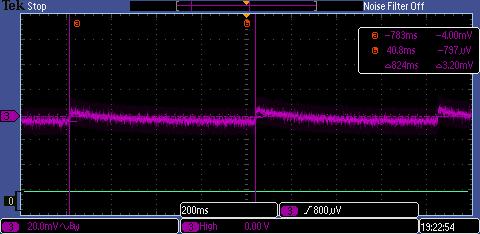
\includegraphics[scale = 0.6]{3Vorgehen/imag/470uF.PNG}
    \caption{Rippelspannung bei Glättung mit 470 $\mu$F Kondensator}\label{kond470uF} 
\end{figure}

Gemäss Ives \textbf{XXXXXX} von EM Microelectronics sollten Kondensatoren der Harvesterschaltung im Bereich von 4.7 $\mu$F liegen, sodass die Energiemanagementschaltung ordnungsgemäss funktioniert.  

Aus diesem Grund wird die Rippelspannung am Ausgangs der Harvesterschaltung mit kleineren Kondensatoren gemessen. Das Messprotokoll befindet sich im Anhang.

\subsubsection*{Messaufbau}
In der gegebenen Harvesterschaltung wird am Kondensator die Spannung mit einem Kathodenstrahloszilloskop (KO) gemesssen. Ausgehend vom bestehenden Kondensator (470 uF), werden danach Elektrolytkondensatoren (Elko) mit den Werten 100 $\mu F $F, 47 $\mu$F und 10 $\mu$F gemessen.

\begin{figure}[h]
    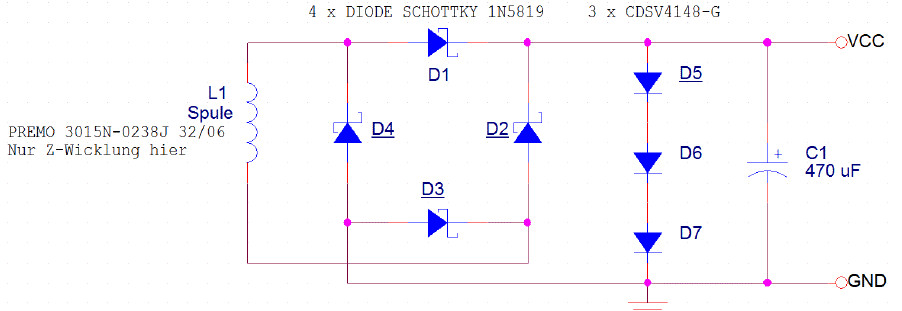
\includegraphics[scale = 0.4]{3Vorgehen/imag/messschaltungHarvesterschaltung.jpg}
    \caption{Messschaltung}
\end{figure}

\subsubsection*{Resultat}

Die Rippelspannung erhöht sich wie erwartet. Vpp beträgt bei 100 uF \textbf{xx} mV, bei 47 uF 28.8 mV (siehe Abbildung \ref{kond47uF}) und bei 10 uF 320 mV (Abbildung \ref{kond10uF}).
 
\begin{figure}
    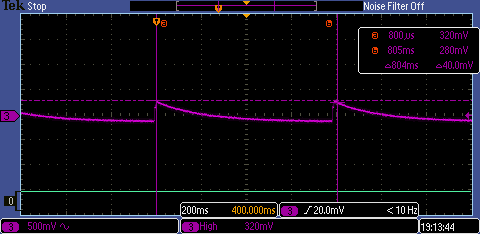
\includegraphics[scale = 0.4]{3Vorgehen/imag/10uF.PNG}
    \caption{Rippelspannung mit 10 uF Kondensator}\label{kond10uF} 
\end{figure}

\begin{figure}
    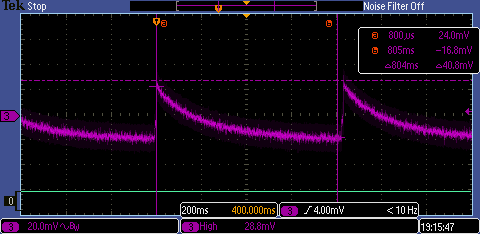
\includegraphics[scale = 0.4]{3Vorgehen/imag/47uF.PNG}
    \caption{Rippelspannung mit 47 uFKondensator}\label{kond47uF} 
\end{figure}


\subsubsection{Messungen Energy Management Board}
In der Projektarbeit findet sich auf S. 36 folgende Abbildung \ref{spannungMachbarkeit} zu den Spannungswerten des Modells der Machbarkeitsstudie.

\begin{tabbing}
    Channel\quad\= Farbe\quad\= Beschreibung\\[0.8ex]
    CH1\> gelb\> Spannung von Harvesterquelle\\
    CH2\> blau\> Spannung am STS--Kondensator\\
    CH3\> violet\> Spannung am LTS--Kondensator\\
    CH4\> grün\> Ausgangsspannung Energiemanagment\\
\end{tabbing}

\begin{figure}
    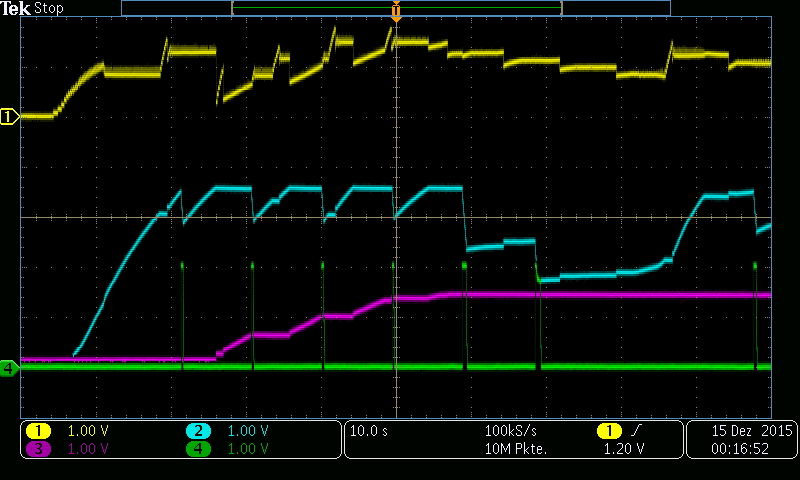
\includegraphics[scale = 0.3]{3Vorgehen/imag/messungPA.png}
    \caption{Spannungswerte Modell der Machbarkeitsstudie}\label{spannungMachbarkeit} 
\end{figure}

Auffällig sind zwei Spannungskurven: Die Spannung des Energieerzeugers. Die Spannungsregelung am Eingang der EMS funktioniert nicht korrekt. Zwischen zwei Regelperioden sollten konstante Spannungen eintreffen (siehe Erklärung in ref). 
Es zeigt sich, dass der LTS nicht geladen wird . Und es zeigt sich, dass das EM-Board nicht zu regulieren beginnt. Damit das Energiemanagement funktioniert, muss der Wer XXXX erreicht werden. Da dieser Wert nicht erreicht wird, passt die Energiemanagementschaltung den Innenwiderstand nicht auf.

Zum korrekten Einstellen des Energiemanagements braucht es eine MaximumPowerPointTracking-Ratio.








\section{Layout Print}

Die Spule ist gegeben.

\subsection{Bauteiloptimierung}
Der Glättungskondensator wird auf 47 uF geändert. Daneben führten nachfolgende Messung zu nachfolgender Bauteiloptimierungen.

\subsubsection{Limiter mit weniger Leckstrom}
Der Limiter in der Machbarkeitsstudie besteht aus 3 Dioden. Die verwendete Dioden haben, wie alle Halbleiterelemente, einen Leckstrom. 

\subsubsection*{Leckstrom Dioden als Limiter}


\subsubsection*{Leckstrom bei LDO}



\subsubsection{Gleichrichter für LowPower}


\section{Energie Management}


\subsection{Energiekalkulation}
EHRV gesammelt >= BLESenden
Zeitkomponente
Energie Harvester braucht länger, verbrauch schneller.

Die Energie der Quelle [$\bar{E_{HRV}} $] muss ausreichen für das Versenden der Datenpakte über Bluetooth smart [$\bar{E_{BLE}}$].

\[\bar{E_{HRV}} \ge \bar{E_{BLE}}  \]


Die durchschnittliche maximale Leistung der Quelle kann aus der Abbildung \ref{MPP_Werte} entnommen werden. Diese basiert auf dem Messprotokoll im Anhang \ref{anhang_messprotokoll_energie_harvester}. 

MAN KÖNNTE. (GEHRÖT ZU OPTIONAL) Da die produzierter Energie von der Fahrgeschwindigkeit abhängt, wird das Energie-System in drei Zustände eingeteilt:

\begin{itemize}
    \item tiefe Geschwindigkeit: 0 - 10 km/h
    \item mittlere Geschwindigkeit: 10 - 20 km/h 
    \item hohe Geschwindigkeit: grösser als 20 km/h 
\end{itemize}



\subsubsection*{Leistungsabgabe Harvester-Schaltung}

\begin{tabular}{|l|l|}\hline \label{MPP_Werte} 
    Geschwindigkeit [km/h] & Maximale Leistung [$\mu W$] \\ \hline
    10 & 74.4 \\ \hline
    20 & unbekannt \\ \hline
    40 & unbekannt \\ \hline
\end{tabular}


Der Energieverbrauch hängt von der Anzahl ausgelesener Daten ab. Wird nur die Geschwindigkeit übermittelt, ist der Verbrauch kleiner, als wenn zusätzlich die Temperatur und die Höhe mitgesendet werden.

\subsubsection*{Energieverbrauch BLE-Packete versenden}
 
\begin{tabular}{|l|l|}\hline \label{Energie_Pakete_Werte} 
    Anzahl Inhalte  & Energieverbrauch [$\mu J$] \\ \hline
    1 & 11000 \\ \hline
    2 & unbekannt \\ \hline
    3 & unbekannt \\ \hline
\end{tabular}

(Für die Zuverlässigkeit der Datenübermittlung wird jeweils dasselbe Paket über drei Kanäle gesendet. Wenn hier \glqq 1 Inhalt versenden \grqq  steht, meint dies, ein Paket über drei Kanäle senden.)

\subsubsection*{Berechnung}

\[\bar{E_{HRV}} = \bar{P} * t \ge \bar{E_{BLE}}  \]
\[\bar{P_{10km/h}} * t = 11 * 10^{-3}  \]
\[74.4 * 10^{-6} * t = 11 * 10^{-3}   \]
\[t = 147 s  \]

\[\bar{E_{HRV}} = \bar{P} * t \ge \bar{E_{BLE}}  \]
\[\bar{P_{10km/h}} * t = 11 * 10^{-3}  \]
\[74.4 * 10^{-6} * t = 11 * 10^{-3}   \]
\[t = 147 s  \]

\subsubsection*{EM BOARD KONZEPT}
Funktion generell beschreiben (im Anhang) 
\subsubsection*{Schwellwerte}
Ausrechnend der schwellwerte
\subsubsection*{Konfigurationen}
Konfigurationseinstellungen



\section{Low Power Einstellungen Sensortag}

Gearbeitet wird mit einem Cortex M3 von TI. 
Grundsätzlich basieren die Bsp. auf RTOS. Wenige für PowerManagement. Das Powermanagement ohne Betriessystem. Wir verwenden dies, weil (gemäss Erfahrungswerte Praxis) mit Betriebsystem mehr Energie braucht).

\subsection{VO: SimpleBroadcast}
- Was ist der Unterschied zum RTOS.
- Was muss gemacht werden.

- Was überprüft werden musste, was gut ist.

Gestartet mit simpleBLE-Projekt von TI mit Einstellungen von Assistenten vom Ines.

\begin{itemize}
    \item Configure ccfg.c to use internal LF RCOSC
    \item Configure WAKE INTERVAL
    \item Configure recharge period to 400ms if WAKE INTERVAL is larger than 400ms(ish)
    \item Configure IO's and set up advertisment payload       
\end{itemize}

Allgemeine Einstellungen in der Konfigurationsdatei ccfg.c:
Vmin = 2.25 V
Imax = 39 mA


Da VSUP bei 1.8 V startet, ist zu überprüfen. 


// RTC wakeup interval
\#define WAKE\_INTERVAL\_MS 		1000
\#define WAKE\_INTERVAL\_TICKS 	WAKE\_INTERVAL\_MS*65536 / 1000


// Advertisment payload length in bytes
\#define ADVLEN 10


Gehen in den Standby modus. Wird eingestellt über die Datei pwr\_ctr.c /h

Dort stehen alle Handlungen, die das System macht, um in den Standby-Modus zu gelangen.

\subsection{V1}


\subsection{V2}


\section{Applikationsentwicklung}

\section{Option 1}






